\section{Select value generation method}
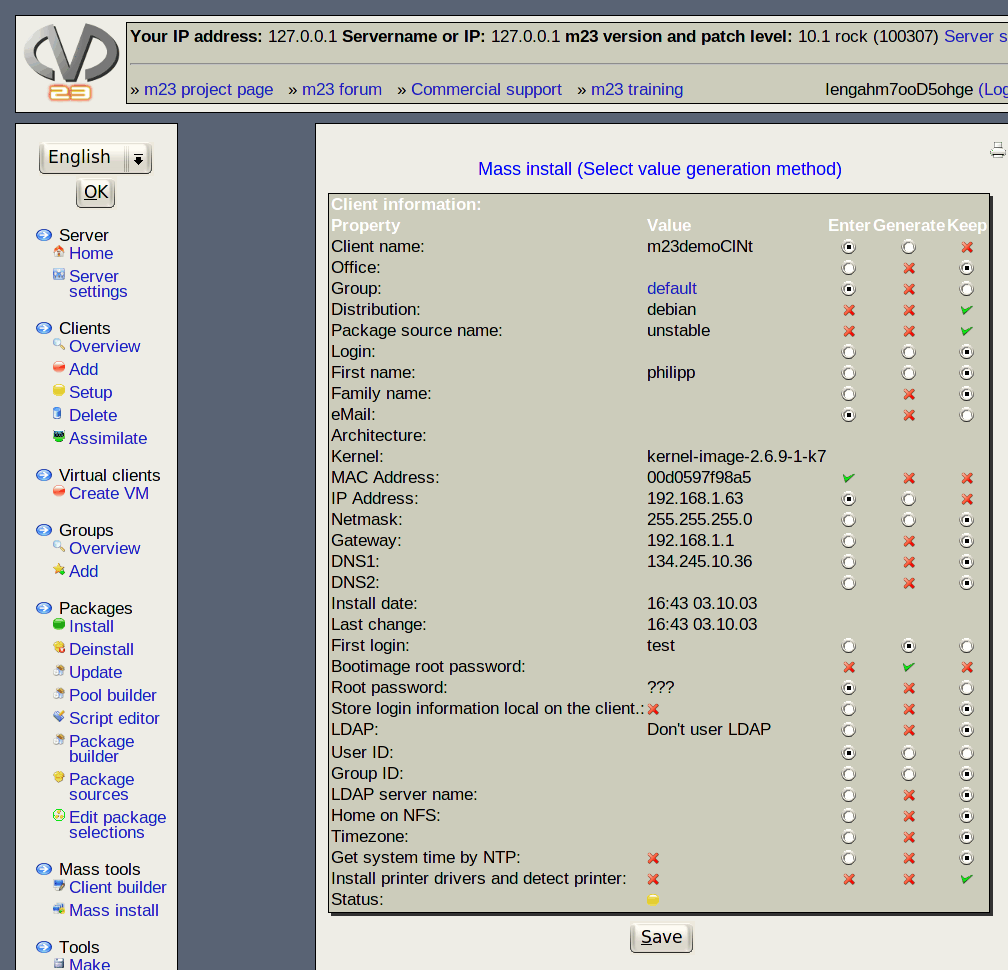
\includegraphics[scale=0.4]{/mdk/doc/manual/screenshots/en/mi_step0.png} \\
Here you can select the method for generation of the needed values.\\
\subsection{There are 3 methods}
\begin{itemize}
\item \textbf{Enter}: The values are entered by hand or read from a file.\\
\item \textbf{Generate}: The values are generated automatically. E.g. it is possible to generate client names with incrementing numbers or IP adressess with unused IP numbers.\\
\item \textbf{Keep}: The value from the "master client" is kept on all clients.\\
\end{itemize}
You don't have the possiblillity to select all 3 methods on every client option. Not selectable options are marked with a red cross. A green check shows that this method is the only one that works for this client option. E.g. it is not possible to generate MAC addresses nor to keep a MAC for all clients. MAC adresses always have to be entered by hand or read from a file.\\
